\documentclass[11pt,a4paper]{article}
\usepackage[margin=2cm]{geometry}
\usepackage{times}
\usepackage{latexsym}

\usepackage{booktabs}
\usepackage{listings}

\usepackage{graphicx}
\usepackage{tikz}
\usepackage{pgfplots}
\usepackage{pgfplotstable}
\usepgfplotslibrary{groupplots}
\pgfplotsset{compat=newest}
\usepackage{siunitx}
\usepackage{amsmath,amssymb,bm,bbm}
\usepackage{datatool}
\usepackage{etoolbox}
\usepackage{stfloats}
\usepackage{amsmath,amssymb,bm,bbm}
\usepackage{datatool}
\usepackage{etoolbox}
\usepackage{stfloats}
\usepackage{filecontents}
\usepackage{enumitem}
\setlist{noitemsep}

\usepackage{microtype}

\widowpenalty10000
\clubpenalty10000

\definecolor{bblue}{HTML}{4F81BD}
\definecolor{rred}{HTML}{C0504D}
\definecolor{ggreen}{HTML}{9BBB59}
\definecolor{ppurple}{HTML}{9F4C7C}
\definecolor{oorange}{HTML}{F08000}

\renewcommand{\topfraction}{0.85}

\lstset { %
    language=C++,
    basicstyle=\footnotesize\ttfamily,
    xleftmargin=0pt
}

\begin{document}

\centering
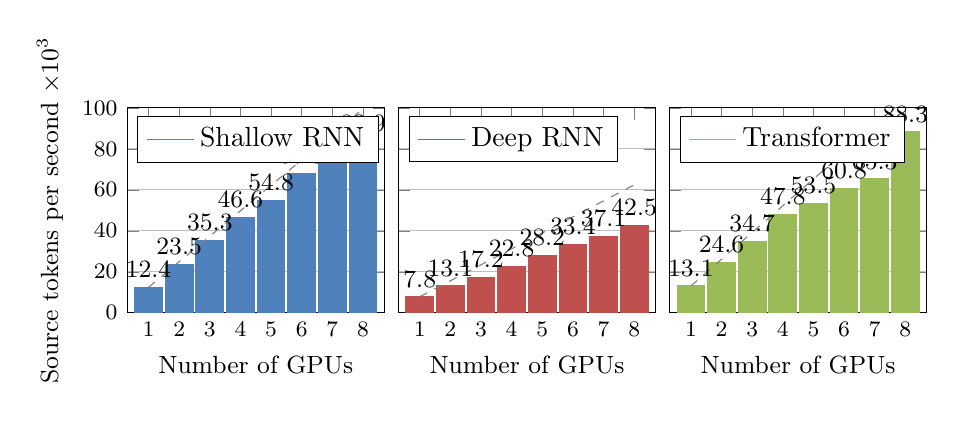
\begin{tikzpicture}
    \begin{groupplot}[
            group style={group size= 3 by 1, vertical sep=1em,
                ylabels at=edge left,
                yticklabels at=edge left,
                xlabels at=edge bottom,
                xticklabels at=edge bottom,
            horizontal sep=5pt},
            ytick scale label code/.code={},
            small, width=0.4\textwidth,
            ymajorgrids,
            xlabel={Number of GPUs}, ylabel={Source tokens per second $\times 10^3$},
            ymin=0, ymax=100000,
            xtick={1 ,2 ,3, 4 ,5, 6, 7, 8},
            legend style={at={(0.04,0.96)},anchor=north west},
        nodes near coords style={font=\small, text=black,/pgf/number format/.cd,fixed zerofill,precision=1}]
        \nextgroupplot[scaled y ticks=base 10:-3]

        \addlegendimage{bblue, refstyle=barplot1}
        \addlegendentry{Shallow RNN}
        \addplot[ybar=0, ybar legend, bblue, fill, visualization depends on={rawy/1e3 \as \scaledy},
        nodes near coords={\pgfmathprintnumber{\scaledy}}] plot coordinates {
        (1, 12444) (2, 23458) (3,35262) (4, 46630) (5, 54765) (6, 67936) (7, 72953) (8, 83855)};
        \label{barplot1}


        \addplot[gray, dashed] plot coordinates {
            (1, 12444) (8, 99552)
        };
        %\legend{shallow, projected};

        \nextgroupplot[scaled y ticks=base 10:-3]
        \addlegendimage{rred, refstyle=barplot2}
        \addlegendentry{Deep RNN}
        \addplot+[ybar=0, ybar legend, rred, mark=none, fill, visualization depends on={rawy/1e3 \as \scaledy},   nodes near coords={\pgfmathprintnumber{\scaledy}}] plot coordinates {
            (1, 7802) (2, 13119) (3, 17230) (4, 22756) (5, 28154) (6, 33374) (7, 37134) (8, 42487)
        };
        \label{barplot2}

        \addplot[gray, dashed] plot coordinates {
            (1, 7802) (8, 62416)
        };

        \nextgroupplot[scaled y ticks=base 10:-3]
        \addlegendimage{ggreen, refstyle=barplot3}
        \addlegendentry{Transformer}
        \addplot+[ybar=0, ggreen, ybar legend, mark=none, fill, visualization depends on={rawy/1e3 \as \scaledy},
        nodes near coords={\pgfmathprintnumber{\scaledy}}] plot coordinates {
            (1, 13059) (2, 24604) (3, 34746) (4, 47834) (5, 53534)
            (6, 60836) (7, 65336) (8, 88283)
        };
        \label{barplot3}

        \addplot[gray, dashed] plot coordinates {
            (1, 13059) (8, 104472)
        };
    \end{groupplot}
\end{tikzpicture}



\end{document}
